% !TEX root=../master.tex
\chapter{GPS-Denied Relative-Pose Estimation}
\label{ch:relative_pose} 

%% TODO: Add related works here
\section{Background and related works}
With each vehicle estimating its own self-pose and body frame velocity, the next step is to estimate the line of sight (LOS) vector between the two vehicles, represented by $\p_{\TwrtH}^\hb$ in \eqref{eq:target_rel_pos}. 
In order to estimate the relative pose between the two vehicles, we assume that the handoff vehicle is receiving measurements of the range between the two vehicles, given by $\xyrange$ where $\xyrange = \norm{\losxy}$.
Because we are measuring the magnitude of the line-of-sight vector, the remaining unknown aspects of the relative pose are the bearing of the LOS vector in the handoff vehicle's navigation frame and the relative heading between the two vehicles. 
We focus primarily on estimating the bearing of the LOS vector, which we represent as $\bearing$. 
We assume that each vehicle is using a calibrated magnetometer that produces a noisy, yet reasonable estimate of global heading, allowing the handoff vehicle to compute the relative heading between the two vehicles, $\relpsifull$.
In \cite{BaiBeard16}, He Bai et al. offer a solution to a similar problem, where the position between the two vehicles is measured and the heading between the two vehicles is estimated using a bank of Kalman Filters. 
We follow a similar approach by using a particle filter to estimate the bearing of the LOS vector, but with a reduced memory and computation footprint.

Agostino Martinelli et al. also offer an observability analysis of estimating the relative pose with a range measurement, showing that the relative pose is observable given that both vehicles have non-zero velocity \cite{MartinelliSiegward05}. 
While the analysis in \cite{MartinelliSiegward05} was performed with 2-dimensional ground robots, we decouple the 3-dimensional problem into relative height and relative position in the $xy$-plane, effectively reducing the bearing estimation to a 2D problem, allowing us to benefit from the observability result. 

\section{State definition}
The goal of the filter is to estimate $\losxy$ measurements of the range between the two vehicles and measurements of each vehicle's altitude.
Because we receive measurements of range directly, we reparameterize $\losxy$ by using polar coordinates for the $xy$-plane. 
This polar-coordinate reparameterization is represented by $\los$, according to
\begin{equation}
    \los = \begin{pmatrix}
    \xyrange \\ \bearing \\ \relzfull
    \end{pmatrix} \;,
\end{equation}
where $\bearing$ is the bearing angle of the LOS vector in the $xy$-plane and $\relzfull$ is the difference in altitude between the handoff and tracking UAVs, given by $z_t - z_h$.

In addition to estimating the LOS vector, we also include the relative heading as a state in the filter to improve upon the noisy measurements from the magnetometers.
Accordingly, the state for the filter becomes
\begin{equation} \label{eq:pf_state}
    \x = \begin{pmatrix} \xyrange \\ \bearing \\ \relzfull \\ \relpsifull \end{pmatrix}
\end{equation} \;.

\section{State Dynamics}
Before discussing the actual filter implementation, it is instructive to first investigate the dynamics of the state, $\x$.
Although the filter uses a polar-coordinate definition for the LOS vector, we begin the derivation of the dynamics using a Cartesian representation for simplicity.

Let $\losxy$ represent the Cartesian LOS vector from the handoff vehicle to the tracking vehicle in the handoff vehicle-1 frame, given by
\begin{align}
    \losxy &= \Rot{i}{\hv}\p_{\TwrtH}^{i} \;,
\end{align}
where $\p_{\TwrtH}^i$ is a NED vector representing the position of the tracking vehicle relative to the handoff vehicle in the inertial frame.

Taking the time derivative, we get
\begin{align}
    \losxy[\dot] &= \Rotdot{i}{\hv}\p_{\TwrtH}^{i} +
                  \Rot{i}{\hv}\dot{\p}_{\TwrtH}^{i} \\
    \label{eq:vhhv}
    &= \Rotdot{i}{\hv}\p_{\TwrtH}^{i} +
       \Rot{\tv}{\hv}\Rot{\tb}{\tv}\vel_{\TwrtI}^{\tb} -
       \Rot{\hb}{\hv}\vel_{\HwrtI}^{\hb} \\
    &= -\skewmat{\angvel_{\HVwrtI}^\hv}\Rot{i}{\hv}\p_{\TwrtH}^{i} +
       \Rot{\tv}{\hv}\Rot{\tb}{\tv}\vel_{\TwrtI}^{\tb} -
       \Rot{\hb}{\hv}\vel_{\HwrtI}^{\hb} \\
    &= -\skewmat{\angvel_{\HVwrtI}^\hv}\p_{\TwrtH}^\hv +
       \Rot{\tv}{\hv}\Rot{\tb}{\tv}\vel_{\TwrtI}^{\tb} -
       \Rot{\hb}{\hv}\vel_{\HwrtI}^{\hb} \\
    \label{eq:losdot}
    &= -\skewmat{\angvel_{\HVwrtI}^\hv}\losxy + \vel_{\TwrtH}^\hv \;,
\end{align}
where $\skewmat{\cdot}$ is the skew-symmetric matrix operator such
\begin{equation}
  \skewmat{\vect{a}} \triangleq \begin{bmatrix}
                                0 & -a_z & a_y \\
                                a_z & 0 & -a_x \\
                                -a_y & a_x & 0
                                \end{bmatrix}.
\end{equation}
Also, because the handoff vehicle-1 frame only differs from the inertial frame by a $z$ rotation, $\angvel_{\HVwrtI}^\hv$ can be interpreted as the rotation about the $z$ axis of the vehicle-1 frame, given by
\begin{align}
    \label{eq:omega_z}
    \angvel_{\HVwrtI}^\hv &= \e_3\e_3^\transpose\Rot{\hb}{\hv}\angvel_{\HBwrtI}^\hb \\
    &= \angvel_{\text{h}z}^\hv \;.
\end{align}

The dynamic equation in \eqref{eq:losdot} essentially has two parts.
The first half of the sum represents the rotational part, which is the relative motion induced by the handoff vehicle's yawing motion.
The second half of the sum represents the translational part, caused by the relative linear velocity between the two vehicles.
For simplicity, we will consider the effect that each of the components have on the polar-coordinate representation separately, then combine them for a final result.

If the handoff vehicle had no rotational motion (e.g. $\angvel_{\text{h}z}^\hv = \mathbf{0}$, the time derivative of the LOS vector would depend entirely on $\vel_{\TwrtH}^\hv$.
The velocity vector can be thought of as having two components---one that is parallel to the LOS vector, representing the radial motion of the tracking vehicle towards and away from the handoff vehicle, and one that is orthogonal to the LOS vector, representing the tangential motion about the current radius at which the tracking vehicle resides (see Figure~\ref{fig:rel_pose_vectors}).

\begin{figure}[hbt]
    \centering
    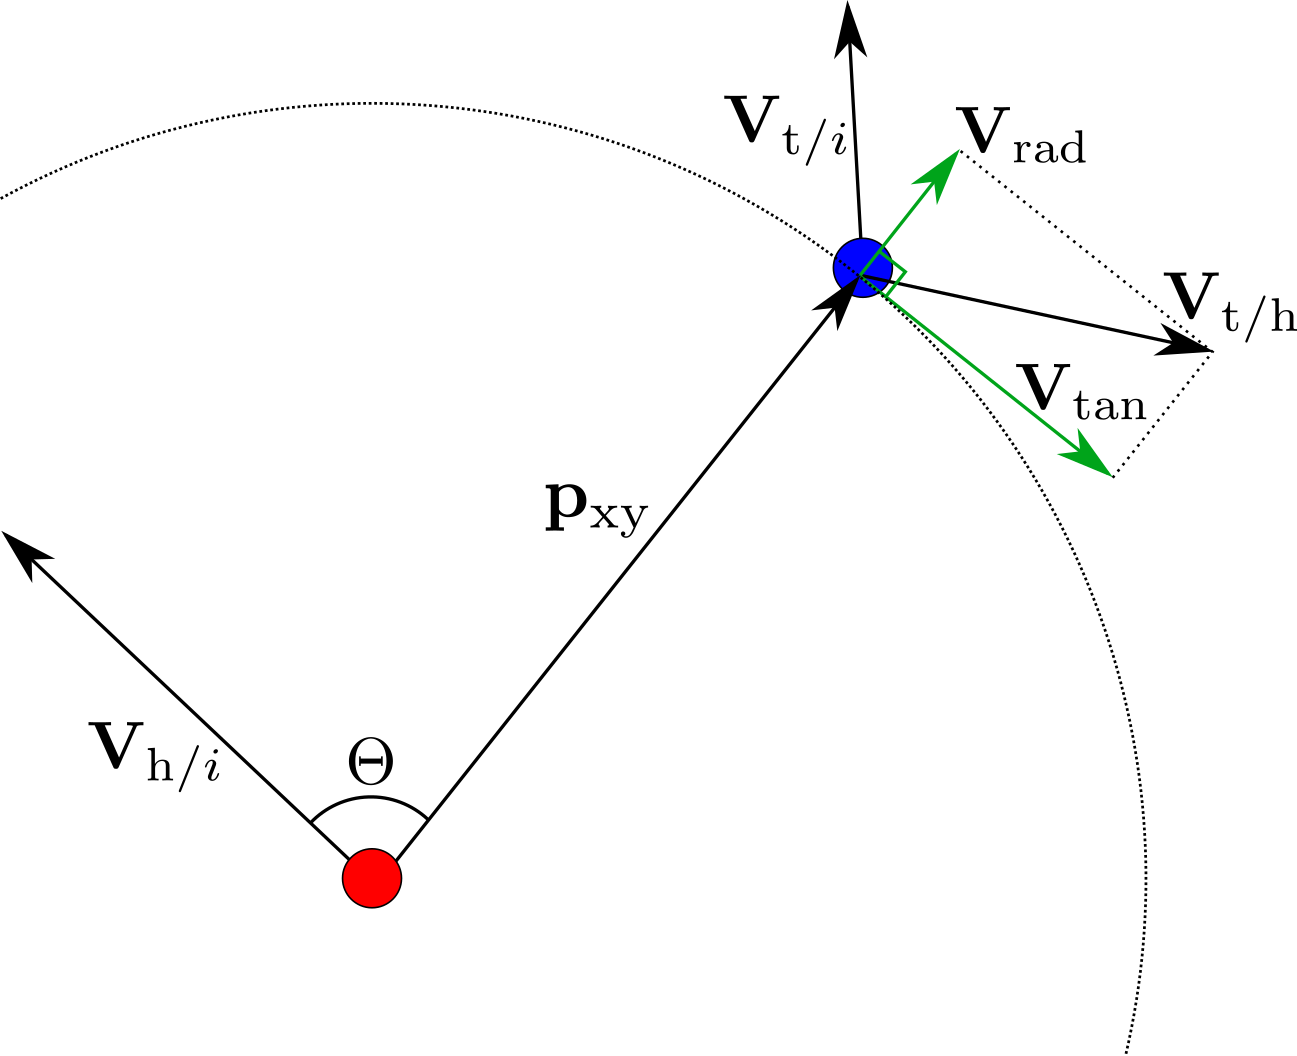
\includegraphics[width=0.5\columnwidth]{figures/rel_pose_vectors}
    \caption{Depiction of relative pose vectors.}
    \label{fig:rel_pose_vectors}
\end{figure}

Using these components, it is simple to derive the polar coordinate dynamics.
The change in range, $\xyrange[\dot]$, depends directly on the radial component according to
\begin{align}
    \xyrange[\dot] &= \norm{\vel_\text{rad}} \\
        &= \frac{\vel_{\TwrtH}^\hv \cdot \pxy}{\norm{\pxy}} \label{eq:rhodot_projection} \\
        &= \vel_{\TwrtH}^\hv \cdot \begin{pmatrix} \cos\bearing \\ \sin\bearing \\ 0 \end{pmatrix} \;,
\end{align}
where $\pxy$ represents the LOS projected onto the $xy$-plane.

The change in bearing can be derived from the tangential component according to
\begin{align}
    \bearing[\dot] &= \frac{\norm{\vel_\text{tan}}}{\xyrange} \\
        &= \frac{1}{\xyrange} \vel_{\TwrtH}^\hv \cdot \begin{pmatrix} -\sin\bearing \\ \cos\bearing \\ 0 \end{pmatrix} \;.
\end{align}
The $z$ component of $\los$ is simply dependent upon the $z$ component of $\vel_{\TwrtH}^\hv$ such that
\begin{equation}
    \relzfull[\dot] = \e_3 \cdot \vel_{\TwrtH}^\hv \;.
\end{equation}

The rotational part of \eqref{eq:losdot} only effects the $\bearing$ dynamics, so the full dynamics of $\los$ become
\begin{align}
    \los[\dot] &= \begin{pmatrix}
        \begin{bmatrix} \cos\bearing & \sin\bearing & 0 \end{bmatrix} \vel_{\TwrtH}^\hv   \\
        \frac{1}{\xyrange} \begin{bmatrix} -\sin\bearing & \cos\bearing & 0 \end{bmatrix} \vel_{\TwrtH}^\hv  - \angvel_{\text{h}z}^\hv \\
        \e_3 \cdot \vel_{\TwrtH}^\hv
        \end{pmatrix} \\
    &= \begin{pmatrix}
    \cos\bearing & \sin\bearing & 0 \\
    -\frac{1}{\xyrange}\sin\bearing & \frac{1}{\xyrange}\cos\bearing & 0 \\
    0 & 0 & 1
    \end{pmatrix} \vel_{\TwrtH}^\hv - \begin{pmatrix} 0 \\ \angvel_{\text{h}z}^\hv \\ 0 \end{pmatrix} \;.
\end{align}

Finally, the dynamics for $\relpsifull$ are simply the difference between the two vehicles' rotation about the inertial $z$ axis, given by
\begin{equation}
    \relpsifull[\dot] = \angvel_{\text{t}z}^\tv - \angvel_{\text{h}z}^\hv \;.
\end{equation}

Accordingly, the time derivative of the filter state, $\x$, becomes
\begin{align} \label{eq:pf_xdot}
\xdot &= \begin{pmatrix}
        \begin{bmatrix} \cos\bearing & \sin\bearing & 0 \end{bmatrix} \vel_{\TwrtH}^\hv   \\
        \frac{1}{\xyrange} \begin{bmatrix} -\sin\bearing & \cos\bearing & 0 \end{bmatrix} \vel_{\TwrtH}^\hv  - \angvel_{\text{h}z}^\hv \\
        \e_3 \cdot \vel_{\TwrtH}^\hv \\
        \angvel_{\text{t}z}^\tv - \angvel_{\text{h}z}^\hv
        \end{pmatrix} \;.
\end{align}

\section{Filter choice}

% - Problem lends itself to particle filter approach
With measurements of the relative heading, relative altitude, and range between the two vehicles, the main goal of the relative pose estimator is to determine the correct value for $\bearing$, the bearing angle of the line of sight (LOS) vector between the two vehicles in the handoff vehicle-1 frame.

This angle is not directly observable with a single time step because we only receive the magnitude of the LOS vector.
Between two measurements, however, we can use the change in range to narrow the possible values of $\bearing$ down to two options.
As seen in \eqref{eq:rhodot_projection}, $\xyrange[\dot]$ can be expressed as the magnitude of the relative velocity projected onto the LOS vector in the $xy$-plane, according to
\begin{align}
    \xyrange[\dot] &= \frac{\pxy \cdot \vrelfull}{\norm{\pxy}}\\
    &= \frac{\norm{\pxy}\norm{\vrelfull}\cos\beta}{\norm{\pxy}}\\
    &= \norm{\vrelfull}\cos\beta
    \;,
\end{align}
where $\beta$ is the angle between the relative velocity vector and the LOS vector, as seen in Figure~\ref{fig:rhodot_vectors}.

\begin{figure}[hbt]
    \centering
    \includegraphics[width=0.5\columnwidth]{figures/rhodot_vectors}
    \caption{Depiction of two possible $\bearing$ values based on $\xyrange[\dot]$}
    \label{fig:rhodot_vectors}
\end{figure}

Solving for $\beta$, we get
\begin{equation}
    \beta = \pm \acos\left(\frac{\xyrange[\dot]}{\norm{\vrelfull}}\right) \;,
\end{equation}
which means that there are two solutions representing valid values for $\bearing$.
Due to this ambiguity of solutions based on subsequent measurements of the range, filters that attempt to propagate the estimated state along a continuous trajectory, such as an EKF, are not well suited to this problem.
Accordingly, we decided to use a particle filter to approximate this split distribution of appropriate $\bearing$ values.
Over multiple time steps, one of the two bearing distributions will move in a direction that coincides with the dynamics while the other will not, allowing us to determine the correct value probabilistically.

\section{Particle filter implementation}
The particle filter consists of $N$ particles, each with a state and dynamics given by Equations~\eqref{eq:pf_state} and \eqref{eq:pf_xdot} respectively.

The inputs to the system are
\begin{equation}
    \u = \pmat{\angvel_h \\ \angvel_t \\ \vhb \\ \vtb \\ \phi_h \\ \theta_h \\ \phi_t \\ \theta_t} \;,
\end{equation}
where $\angvel_h$ and $\angvel_t$ represent angular velocities from the IMU, $\vhb$ and $\vtb$ are body-frame airspeed vectors from the self-pose filter computed according to \eqref{eq:vair_vec}, and $\phi$ and $\theta$ angles are the estimated roll and pitch angles from the self-pose filter, respectively.

At each time step the state of each particle is propagated according to the dynamics in Equation~\eqref{eq:pf_xdot} with
\begin{align}
    \vrelfull &=\Rot{\tv}{\hv}\Rot{\tb}{\tv}\vel_{\TwrtI}^{\tb} -
       \Rot{\hb}{\hv}\vel_{\HwrtI}^{\hb} \\
       &= \Rot{\relpsi}{}\Rot{\theta_t}{}\Rot{\phi_t}{}\vel_{\TwrtI}^{\tb} -
       \Rot{\theta_h}{}\Rot{\phi_h}{}\vel_{\HwrtI}^{\hb}\;,
\end{align}
and
\begin{align}
    \angvel_{jz}^{j\text{v1}} &=
    \e_3\e_3^\transpose\Rot{j\text{b}}{j\text{v1}}\angvel_{j\text{b}/i}^{j\text{b}} \\
    &= \e_3\e_3^\transpose\Rot{j\theta}{}\Rot{j\phi}{}\angvel_{j\text{b}/i}^{j\text{b}}\;,
\end{align}
where
\begin{align}
        \label{eq:R_psi}
    \Rot{\psi}{} &= \pmat{
        \cos\psi & -\sin\psi & 0 \\
        \sin\psi & \cos\psi & 0 \\
        0 & 0 & 1
    }\;, \\
        \label{eq:R_theta}
    \Rot{\theta}{} &= \pmat{
        \cos\theta & 0 & \sin\theta \\
        0 & 1 & 0 \\
        -\sin\theta & 0 & \cos\theta
    }\;, \\
        \label{eq:R_phi}
    \Rot{\phi}{} &= \pmat{
        1 & 0 & 0 \\
        0 & \cos\phi & -\sin\phi \\
        0 & \sin\phi & \cos\phi
    }\;,
\end{align}
and
\begin{equation}
    \e_3 = \pmat{0 \\ 0\\ 1}\;.
\end{equation}

% - Define measurements and measurement model
The measurement for the filter is composed of range, relative altitude, and relative heading and is defined as
\begin{equation}
    \y = \pmat{\range \\  \relz \\ \relpsi}\;.
\end{equation}
Note that the $[\;]_\text{rel}$ notation is used here in place of $[\;]_{\TwrtH}^{\hv}$ for notational simplicity.

Using the current estimated state of each particle, $\hat{\x}^i_k$, at time step $k$, we construct an estimated measurement, $\y[\hat]$, such that
\begin{equation}
    \y[\hat]^i_k = \pmat{\sqrt{{\xyrange[\hat]}^2 + {\relz[\hat]}^2} \\ \relz[\hat] \\ \relpsi[\hat]}\;.
\end{equation}

Let $\mathbb{Y}\sim \mathcal{N}(\y, \Q)$ represent a multivariate Gaussian distribution centered about $\y$ with covariance $\Q$ and let $f_{\mathbb{Y}}$ be the log PDF of $\mathbb{Y}$.
The weight for each particle is obtained using the softmax function according to
\begin{equation} \label{eq:softmax}
    w^i_k = \frac{\exp\left(f_\mathbb{Y}(\y[\hat]^i_k)\right)}{\sum\limits_{j=1}^{N}\exp\left(f_\mathbb{Y}(\y[\hat]^j_k)\right)}\;,
\end{equation}
where $w^i_k$ represents the weight of the $i$-th particle at time step $k$.
In practice, we use the ``log-sum-exp trick'' for computational stability by subtracting off the maximum log probability, according to
\begin{equation} \label{eq:logsumexp}
    w^i_k = \frac{\exp\left(f_\mathbb{Y}(\y[\hat]^i_k) - \max\limits_l f_\mathbb{Y}(\y[\hat]^l_k) \right)}
    {\sum\limits_{j=1}^{N}\exp\left(f_\mathbb{Y}(\y[\hat]^j_k) - \max\limits_l f_\mathbb{Y}(\y[\hat]^l_k) \right)}\;.
\end{equation}
Equations~\eqref{eq:softmax}~and~\eqref{eq:logsumexp} are mathematically equivalent, but subtracting off the maximum before exponentiating the log probabilities reduces the chance of underflow for low-probability values.

The particles are then resampled with probability proportional to their weights.
However, to reduce particle deprivation and minimize the chance of throwing away good particles, we employ two techniques.
The first is low-variance resampling, which is described in detail in \cite{ThrunBurgardFox06}.
Because the resampling step is a stochastic process, it is possible to lose good particles simply by not resampling them.
Low-variance resampling helps to deal with this challenge by using a random seed to sample from the particles in a more systematic fashion, reducing the probability that particles with higher weights will be lost.

The second technique employed is selective resampling based on the number of effective particles.
This method is described in \cite{GrisettiStachnissBurgard09} and involves resampling only when the number of effective particles drops below a set threshold, such as $\frac{2N}{3}$.
The number of effective particles is estimated by
\begin{equation}
    N_\text{eff}={\frac{1}{\sum\limits_{i=1}^{N} {(w^{i})}^{2}}}\;,
\end{equation}
and is inversely proportional to the variance of the weights.
If the particles very closely match the true distribution, then the particles will have similar weights and low variance.
This would cause $N_\text{eff}$ to be high, which would allow the system to propagate the distribution without the need to resample.
Over time, if the particles became more diffused and the variance of the weights increases, then the number of effective particles would drop below the threshold and new particles would be resampled in an effort to improve the current approximation of the distribution.
By resampling only when $N_\text{eff}$ is below the threshold, the chance of eliminating good particles is reduced.

In order to perform selective resampling, it is important to update the weights of the particles at each successive time step between resampling.
This can be done according to
\begin{equation}
    w^i_{k+1} = \eta w^i_k f_\mathbb{Y}(\y[\hat]^i_{k+1})\;,
\end{equation}
where $\eta$ is a normalization constant.
After the particles are resampled, all weights are reset to $\frac{1}{N}$.

\section{Results} \label{sec:rel_pose_results}
The relative pose particle filter was tested in simulation using simulated IMU, airspeed, altitude, magnetometer, and range measurements, each with added Gaussian noise.
In general, the relative pose estimate converged quickly and provided a sufficiently accurate estimate for the handoff UAV to locate the target and insert into a similar orbit.
As expected, the particle filter displayed a bimodal distribution before converging onto the proper bearing angle as shown in Figure~\ref{fig:particle_filter}.

\begin{figure}[hbt]
  \centering
  \includegraphics[width=\columnwidth]{figures/particle_filter}
  \caption{\textit{Top left}: particles are initialized uniformly across all bearing angles; \textit{Top right}: particles begin to split into a bimodal distribution; \textit{Bottom left}: particles are grouped in two distinct clusters, but with more particle density around the correct bearing; \textit{Bottom right}: the particles consolidate and center around the true value}
  \label{fig:particle_filter}
\end{figure}

Figure~\ref{fig:theta_convergence} shows the estimate of the bearing diverging slightly, then converging sharply as the particles finally consolidate completely around the correct value.
After the particles consolidate, they remain centered around the true value and the estimate of $\Theta$ tracks well.

\begin{figure}[hbt]
  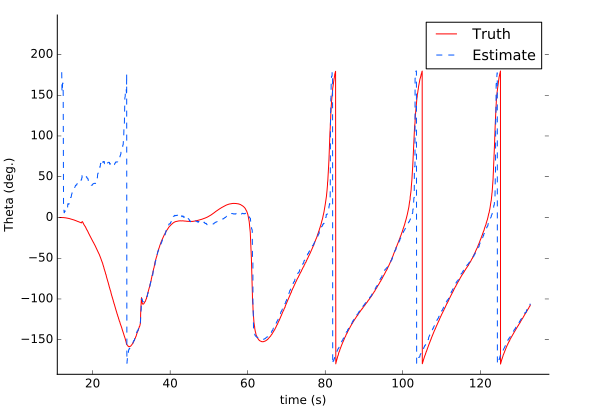
\includegraphics[width=\columnwidth]{figures/Theta_convergence}
  \caption{Plot of $\Theta$ estimate; diverges slightly as particles split into bimodal distribution, then converges sharply as particle consolidate around the true value.}
  \label{fig:theta_convergence}
\end{figure}

\begin{figure}[hbt]
  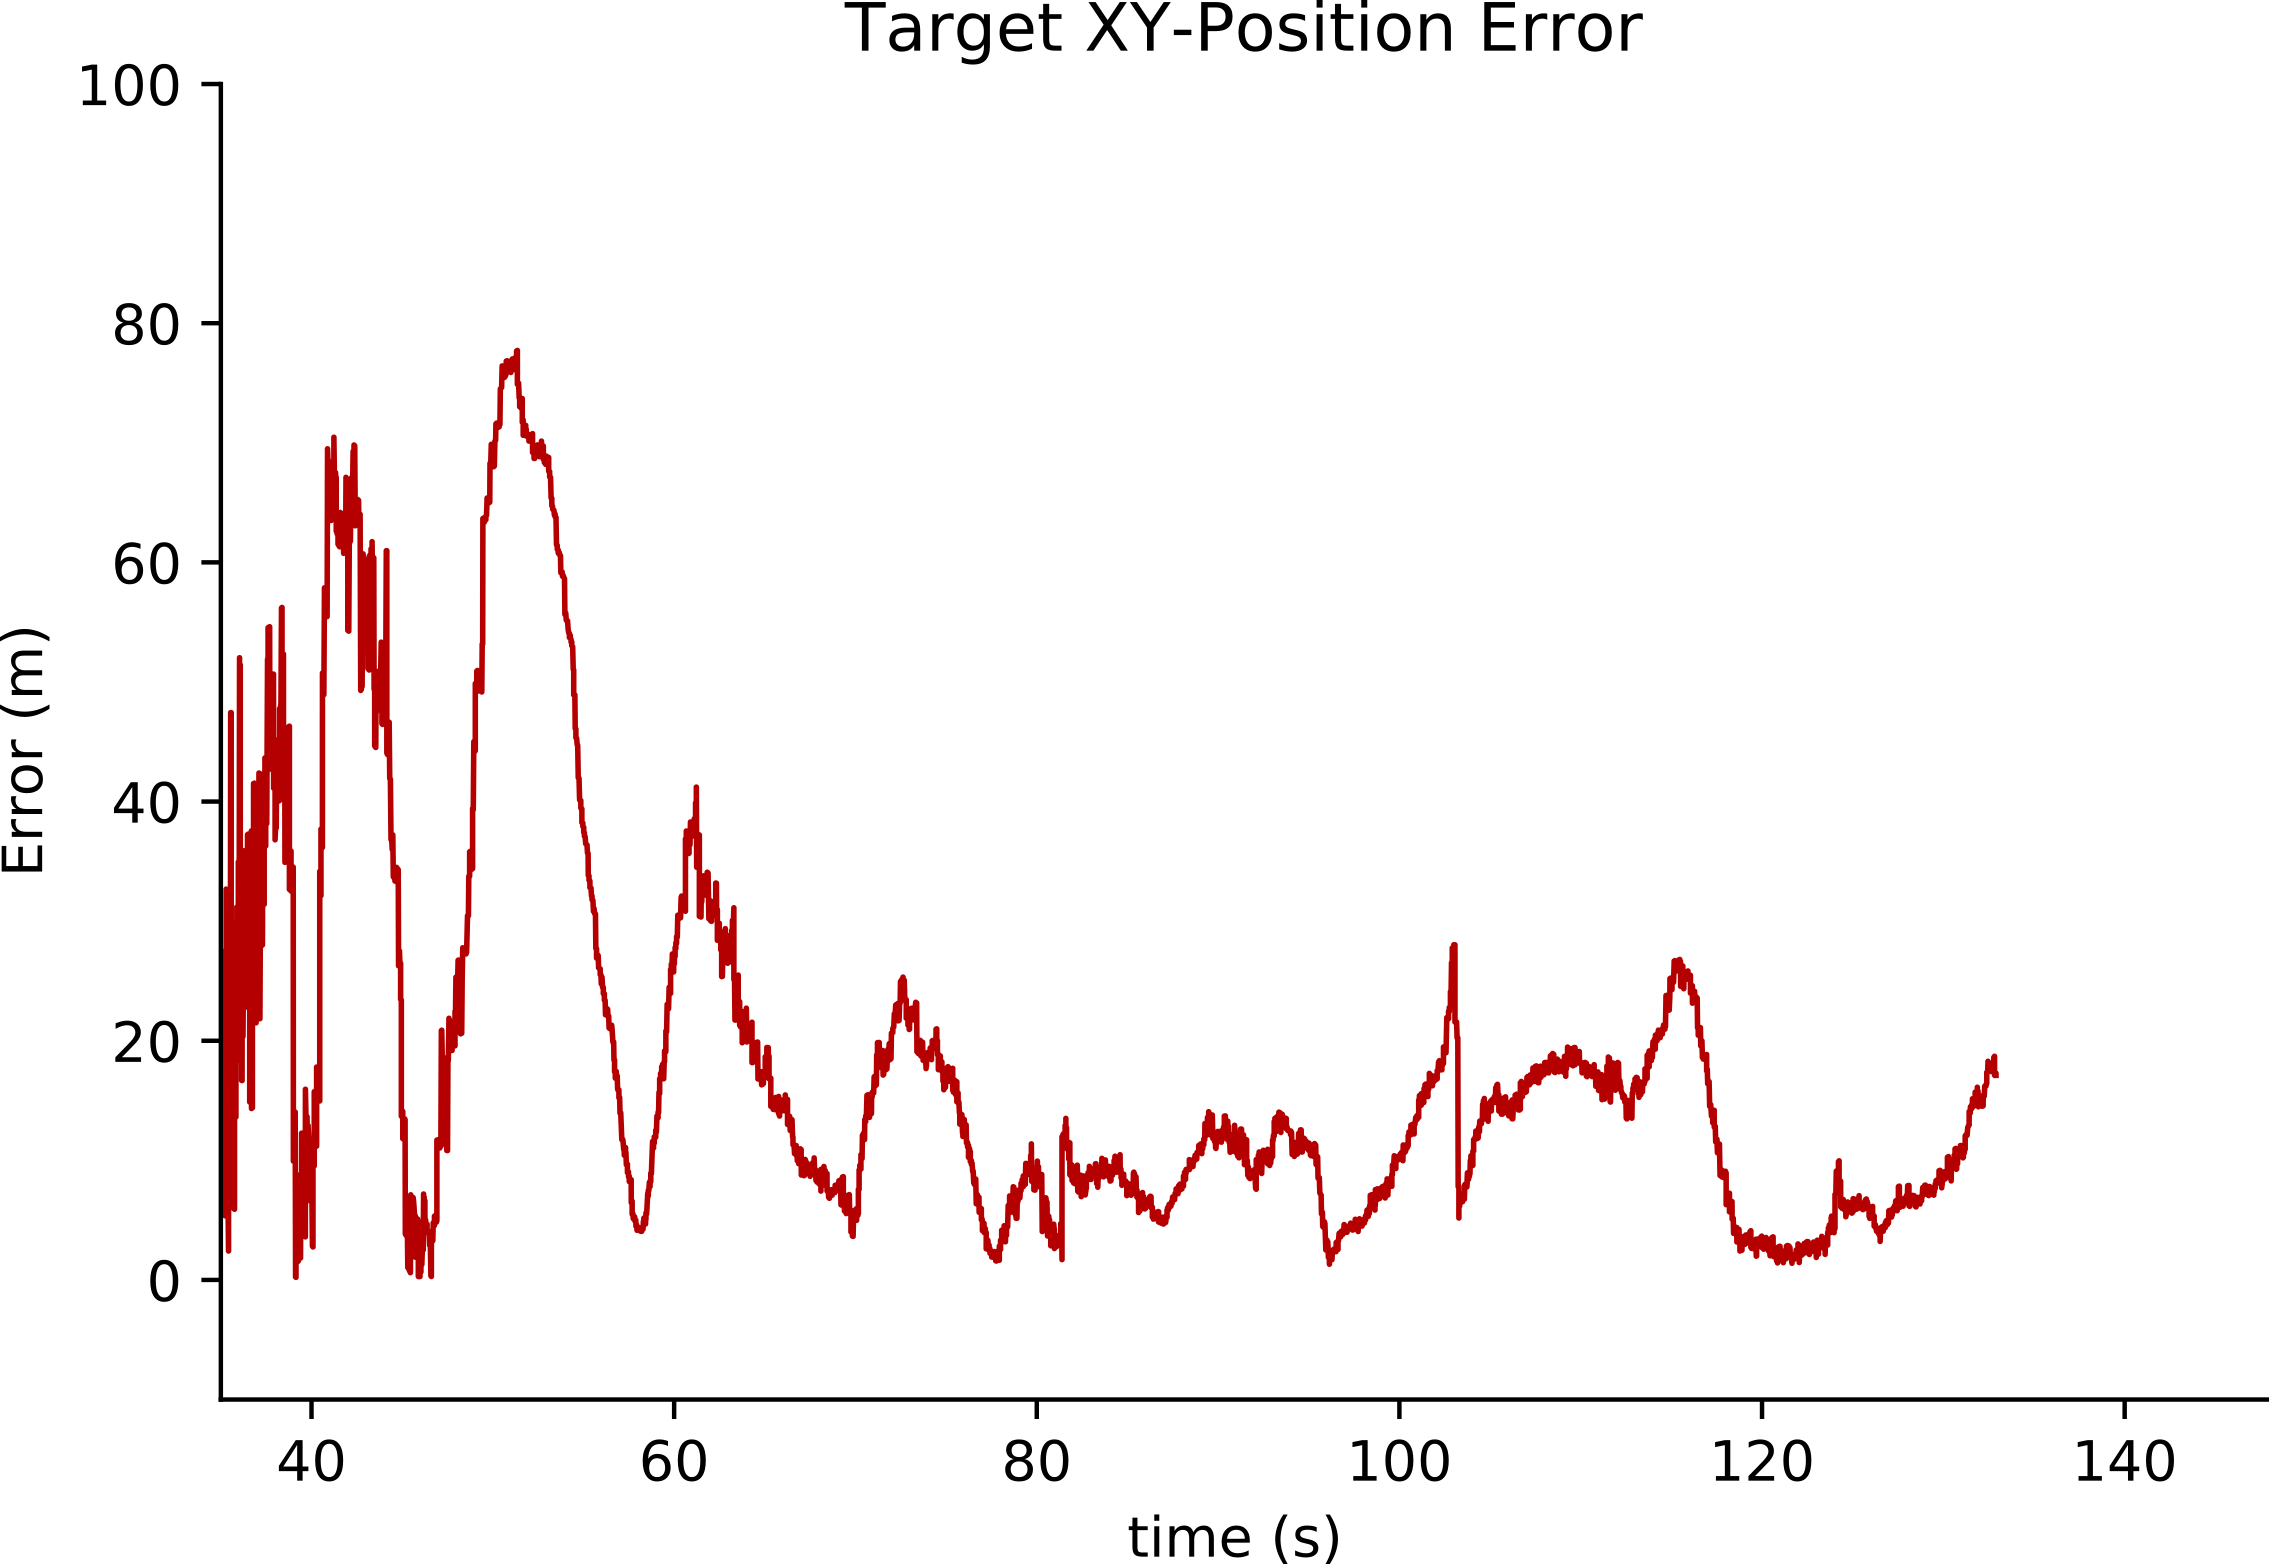
\includegraphics[width=\columnwidth]{figures/target_error}
  \caption{Plot of estimated target $xy$-position error.}
  \label{fig:target_los_error}
\end{figure}

We observed that because the estimated line of sight is parameterized using angle and magnitude and because the range between the two vehicles is often large, small errors in the bearing angle estimate can lead to large errors in the $xy$-plane.
Accordingly, the relative pose estimate is not ideal for obtaining a fine-tuned estimate of the target's position.
However, it does serve it's intended purpose well, providing a reasonable and quickly converging estimate of the relative pose, which allows us to get a good estimate of the target's position to be used in the orbit control.
As seen in Figure~\ref{fig:target_los_error}, after the relative pose estimate begins to converge, the target LOS error can still be as high as 80 meters, but over time, it remains near or below 20 meters.
This level of accuracy is sufficient to locate the target and retain it in the field of view, allowing the handoff UAV to utilize visual information to perform the handoff with greater confidence.

